% This is LLNCS.DEM the demonstration file of
% the LaTeX macro package from Springer-Verlag
% for Lecture Notes in Computer Science,
% version 2.4 for LaTeX2e as of 16. April 2010
%
\documentclass{llncs}
%\documentclass[runningheads]{llncs}

% *** GRAPHICS RELATED PACKAGES ***
\usepackage{graphicx}
% declare the path(s) where your graphic files are
\graphicspath{{./Figs/}}
% and their extensions so you won't have to specify these with
% every instance of \includegraphics
\DeclareGraphicsExtensions{.pdf,.jpeg,.png}

%% ------ Packages added by pete ------ %%
%% ------ packages for authors format  ------ %%
\usepackage[misc]{ifsym}
\usepackage{bbding}
\usepackage{url}

\urldef{\mailsb}\path|{yuwenping}@mail.nankai.edu.cn|
\urldef{\mailsa}\path|{zhangjz, xujd, xuyw}@nankai.edu.cn|
%% ------ packages for authors format  ------ %%

%% ------ packages for subfigures  ------ %%
\usepackage[caption=false,font=footnotesize]{subfig}
%\usepackage{caption}
%\usepackage[justification=centering]{caption}

%% ------ packages for algorithm expressed with the pseudocode  ------ %%
\usepackage{algorithm}
%\usepackage{algorithmic}
\usepackage{algcompatible}

%% ------ packages for list  ------ %%
%\usepackage{enumitem}% http://ctan.org/pkg/enumitem


%% ------ typesetting with little spacing ------ %%
%%% Save the class definition of \subparagraph
%\let\llncssubparagraph\subparagraph
%%% Provide a definition to \subparagraph to keep titlesec happy
%\let\subparagraph\paragraph
%%% Load titlesec
%\usepackage[compact]{titlesec}
%%% Revert \subparagraph to the llncs definition
%\let\subparagraph\llncssubparagraph

\begin{document}

%%
%\mainmatter              % start of the contributions
%
\title{Motion Trajectory Sequence-Based Map Matching Assisted Indoor Autonomous Mobile Robot Positioning}
%J
\titlerunning{MTTSMatch}  % abbreviated title (for running head)
%                                     also used for the TOC unless
%                                     \toctitle is used
%
%%\author{Wenping Yu\inst{1}}

\author{Jianzhong Zhang$^1$ $^($\Envelope$^)$ \and Wenping Yu$^2$ \and Jingdong Xu$^1$ \and Yuwei Xu$^1$}
%
\authorrunning{Wenping Yu et al.} % abbreviated author list (for running head)
%
%%%% list of authors for the TOC (use if author list has to be modified)
\tocauthor{Wenping Yu}
%
\institute{College of Computer and Control Engineering, Nankai University, Tianjin, China\\
$^1$\mailsa\\
$^2$\mailsb\\}


\maketitle              % typeset the title of the contribution

\begin{abstract}

Position information is one of basic elements for context awareness of autonomous mobile robots. This paper studies the positioning algorithm of autonomous mobile robots suitable for search and rescue in dark building corridors and underground mine tunnels when an emergency occurs, and proposes a novel map matching aided positioning algorithm based on Hidden Markov Model. This algorithm does not rely on a camera, and only uses the inertial sensors installed in mobile robot and the indoor map to realize the fusion of dead reckoning and map matching. Firstly, it detects the position-related motion postures during the motion process, and then the motion trajectory is divided into a sub-trajectory sequence. By matching the sub-trajectory sequence with the indoor map, the proposed algorithm achieves tracking and positioning of mobile robots. In order to verify the effectiveness of our proposed algorithm, this paper adopts four-wheel differentially driven robot to conduct experimental analysis in an actual indoor scenario. The experimental results show that compared with the traditional dead reckoning technology, this algorithm can distinctly reduce the average positioning error of mobile robot, and it is robust to heading angle and acceleration noises within a certain error range.

\keywords{Mobile Robot \and Indoor Positioning \and Hidden Markov Model \and Motion Pattern Detection.}
\end{abstract}
%
\section{Introduction}
%
With the advancement of artificial intelligence, network and sensor technologies, the research and application of autonomous mobile robots have made remarkable progress in recent years. Indoor autonomous mobile robots are increasingly integrated into people's daily lives \cite{Garcia2007The}. Autonomous mobile robots can be extensively used not only in modern intelligent warehouses, home services and many other aspects, but also in corridors of complex buildings, tunnels of subway and underground mines when accidents occur. Therefore, the research of indoor autonomous mobile robot technology has gradually become a hot topic, and many domestic research institutes such as Tsinghua University, Harbin Institute of Technology, Nankai University and South China University of Technology are committed to the research and development of indoor autonomous mobile robots \cite{Wu2005Robust,Wu2015A,Yang2015An,yuan2009sprb,yuningbo2017RGBDbae}. The autonomous positioning of the mobile robot is a process in which the robot autonomously determines its position in the working environment, and is one of the most basic problems in improving the autonomous capabilities of the mobile robot.

In terms of outdoor positioning, the Global Positioning System (GPS) has become a widely used positioning technology for mobile robots. However, in terms of indoor positioning, due to the blocking and interference of GPS signals by the external walls of buildings and indoor complex electromagnetic environment, there is no universal solution to the positioning problem of indoor mobile robots \cite{Bachrach2011RANGE,bao2013indoor}. Currently, researchers have proposed a variety of positioning methods for indoor autonomous mobile robots, including navigation beacon-based positioning \cite{Tang2014multiary}, computer vision-based positioning \cite{lu2015visual,gao2017unsupervised}, dead reckoning positioning \cite{kim2015dead}, map matching positioning \cite{grisetti2007improved,cheng2015topological} and simultaneous localization and mapping (SLAM) \cite{de2014feature,havangi2014square}, and so on. Positioning techniques based on navigation beacons rely on a series of deployed feature signals to provide stable and accurate location information, but require high deployment and maintenance costs. Dead reckoning technique uses inertial sensors or encoders to provide relatively accurate positions over short distances, but exists cumulative error that gradually increases as the distance travels, and the robot's starting point needs to be known in advance. Map matching positioning uses known indoor maps to construct topological maps, feature maps, and other abstract maps, and then the position of the mobile robot is obtained by matching the robot motion trajectory with the indoor maps. The real-time performance of map matching is relatively poor according to its realization principle. The SLAM technology has unique advantages in the face of unknown environments and can provide indoor floor plans or 3D maps while providing positioning \cite{richter2018bayesian}. However, this method requires mobile robots equipped with more complex sensor devices, such as infrared, ultrasonic radar and RGB-D vision systems. Therefore, it has higher implementation cost.

Corridors of buildings, subway station tunnels and underground mines often have complex passageways, similar to “mazes”. In the event of an accident such as a fire, the power supply is damaged, the communication infrastructure become unusable and smoke and dust cause the lack of indoor lighting, and so on. All these situations pose challenges for the positioning of indoor autonomous mobile robots. Due to limitations in working environment or deployment conditions, it is difficult to establish visual or wireless navigation beacons in advance. Therefore, positioning technology based on navigation beacons is not suitable; the influence of high temperature and smoke on the indoor environment makes it difficult for cameras to provide image information, visual positioning technology fails; the timeliness of SLAM technology can not meet the urgent need for time factors in the above scenarios. In response to these problems, this paper introduces a hidden Markov model (HMM) based map matching algorithm that does not rely on a camera, only uses inertial sensors (accelerometers, gyroscopes, and magnetometers) installed in autonomous mobile robots and known indoor maps to effectively track and position mobile robots.

%In summary, this paper's mainly contributions are as follows:
%\vspace{-10pt}
%\begin{itemize}
%	\setlength{\parskip}{0pt} 
%	\setlength{\itemsep}{0pt plus 1pt}
%	\renewcommand{\labelitemi}{$\vcenter{\hbox{\tiny$\bullet$}}$}
%	\item we present the architecture of AiFiMatch: a map matching algorithm based on activity detection and crowd-sourced Wi-Fi.
%	\item we present the architecture of AiFiMatch: a map matching algorithm based on activity detection and crowd-sourced Wi-Fi.
%\end{itemize}
%\vspace{-8pt}

%In summary, this paper's mainly contributions are as follows:
%\begin{itemize}[noitemsep,topsep=0pt]
%	\renewcommand{\labelitemi}{$\vcenter{\hbox{\tiny$\bullet$}}$}
%	\item we present the architecture of AiFiMatch: a map matching algorithm based on activity detection and crowd-sourced Wi-Fi.
%	\item we present the architecture of AiFiMatch: a map matching algorithm based on activity detection and crowd-sourced Wi-Fi.
%\end{itemize}

The remainder of this paper is organized as follows: Section II introduces the robot motion model, the overview of proposed algorithm and its preprocessing components. Then, we detail the proposed HMM-based map matching algorithm in Section III. Section IV shows the experimental results and analysis. Finally, Section V concludes this paper.

\section{Robot Motion Model and Positioning Method}

In the field of indoor autonomous mobile robot positioning, dead reckoning technology and map matching technology have a good complementarity. This paper proposes a map matching-assisted positioning method based on motion trajectory sequence of mobile robot to realize the fusion of the above two technologies. The positioning algorithm uses stairs and corridor corners in the indoor environment as virtual landmarks. When the mobile robot passes through these landmarks, the inertial sensor data will show a specific pattern. Therefore, in this paper, the above landmarks are called posture-related positions. When the robot's movement distance is short, the dead reckoning technology can give the real-time position of the robot. When the robot's movement distance is long, the robot's motion trajectory can be divided into multiple sub-trajectories according to the landmarks, consecutive sub-trajectories form sub-trajectory sequence. With the help of HMM model, the above sub-trajectory sequence can be matched to the corresponding road in the indoor map, and then the position estimation of the mobile robot is given. Further, when the robot's motion trajectory is long enough, the absolute position of the mobile robot can still be estimated even without knowing the robot's starting point.

This section firstly introduces the relevant modules and simplified motion models of the four-wheel differential-driven autonomous mobile robot used in subsequent experiments, and then derives the dead reckoning technology based on the motion model. Then the overall architecture of the fusion positioning method proposed in this paper is introduced. And the indoor map abstraction module, the final description of the mobile robot motion gesture recognition and use of the four-wheel differential drive robot designed in this paper to conduct a related pre-experiment. The trajectory matching technology based on Hidden Markov Models is the core module of the positioning method, which will be discussed in detail in the next section.

\subsection{Robot Motion Model and Its Dead Reackoning Principle}

In this paper, a four-wheel differentially driven wheeled mobile robot is used to study the positioning problem of autonomous mobile robots in indoor environment. The driving motor is a DC motor. The two driving motors on one side are connected in reverse parallel and use the L298N motor driving module. Control the DC motor, and the mobile robot adopts the Raspberry Pi second-generation B-board (B.V1.2) as the main control chip. According to the driving mode of the mobile robot, the movement models of the two wheels on each side of the wheeled robot are the same. Therefore, the movement model of the mobile robot can be simplified to a left and right two-wheel differential driving mode. Figure \ref{fig-model-dr} (a) shows the mobile robot. The simplified model, where (x, y) is the position coordinate of the mobile robot in the global coordinate system, $\Theta$ is the included angle between the mobile robot and the true north direction, ie the heading angle.

\begin{figure}[!htbp]
	\centering
	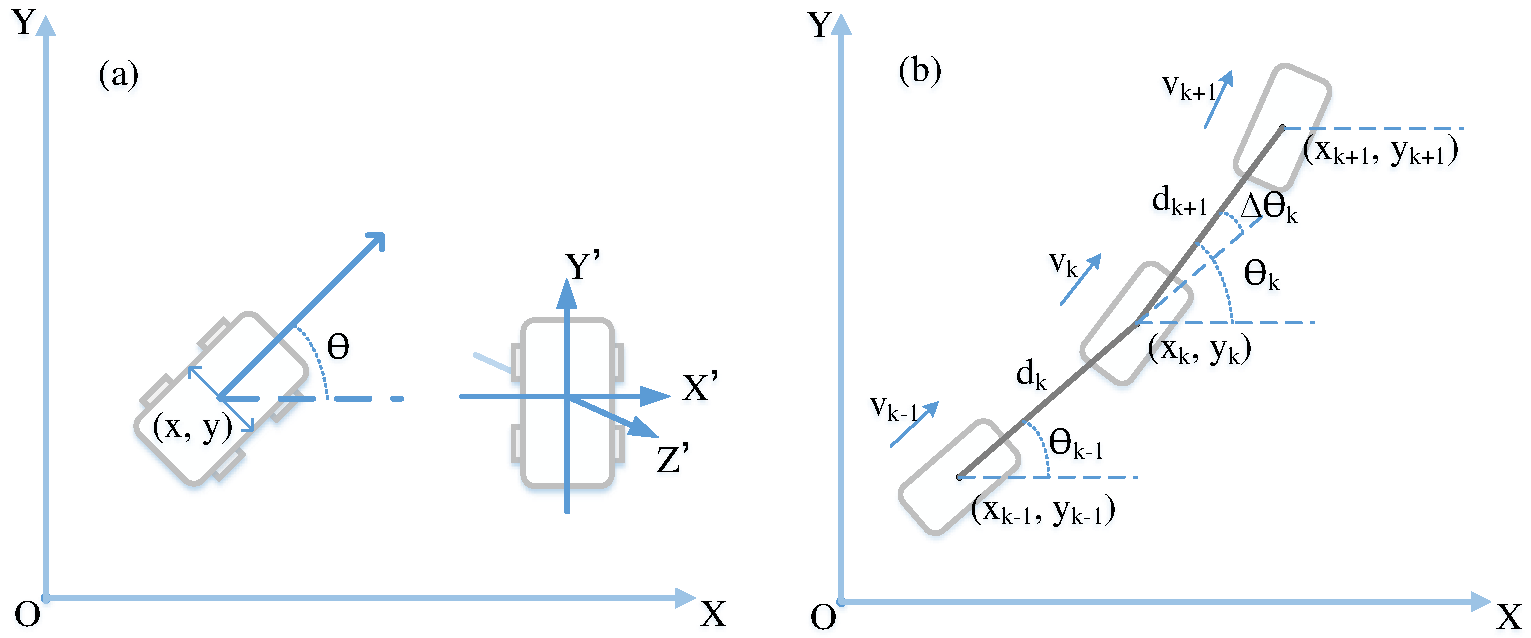
\includegraphics[width=4.7in]{RobotMatch-MotionModel}
	\caption{Simplified motion model and its dead reckoning principle for four-wheel differentially driven robot. (a) Motion model and self coordinate system. (b) Dead reckoning in the global coordinate system.}
	\label{fig-model-dr}
\end{figure}

Dead reckoning technology is widely used in the positioning of indoor autonomous mobile robots, and is particularly suitable for short-range positioning. The autonomous mobile robot used in this article has a built-in digital compass, three-axis accelerometer and gyroscope. The digital compass gives the initial attitude of the mobile robot. The accelerometer and the gyroscope can measure the movement acceleration and rotation angular velocity of the mobile robot, and then pass it. Integral operation can calculate the distance and heading change of the mobile robot, and then analyze the latest position and attitude of the mobile robot.

In order to determine the position and attitude of the mobile robot in the plane and establish the global right angle coordinate system $OXY$, it may be assumed that the initial position $(x_0, y_0)$ is the origin of the coordinates and the initial attitude is the positive direction of the $X$-axis. Then the position and posture of the K time mobile robot can be expressed by vector. In the current moment, the instantaneous velocity of the mobile robot is represented by the angle between the moving direction of the mobile robot and the positive direction of the $X$-axis, and the transverse ordinates of the mobile robot in the global coordinate system, as shown in Figure \ref{fig-model-dr} (b). When the update cycle of sensor data is very small, if the update cycle of the sensor is about 5 milliseconds in this paper, in one cycle, the trajectory of the mobile robot can be approximated to a straight line, then the position of the K time mobile robot can be recursively obtained by the Equation \ref{equ_dr}.

\begin{equation}
\label{equ_dr}
\left( {\begin{array}{*{20}{c}}
	{{v_k}}\\
	{{\theta _k}}\\
	{{x_k}}\\
	{{y_k}}
	\end{array}} \right) = \left( {\begin{array}{*{20}{c}}
	{{v_{k - 1}}}\\
	{{\theta _{k - 1}}}\\
	{{x_{k - 1}}}\\
	{{y_{k - 1}}}
	\end{array}} \right) + \left( {\begin{array}{*{20}{c}}
	{0.5({a_{k - 1}} + {a_k})\Delta t}\\
	{0.5({\omega _{k - 1}} + {\omega _k})\Delta t}\\
	{{d_k}\cos {\theta _{k - 1}}}\\
	{{d_k}\sin {\theta _{k - 1}}}
	\end{array}} \right),k \ge 1
\end{equation}

where the time interval from the $k-1$ time to the $k$ moment, if the sensor fixed the data update period, also represents the update period, indicating the instantaneous acceleration in the direction of the moving robot at the time of $k$, which can be measured by the $Y$-axis component of the accelerometer, indicating the angular velocity of the heading angle at the $k$ time of the moving robot. It can be measured by the $Z$-axis of the gyroscope, and indicates the movement distance of the mobile robot from $k-1$ to $k$. It can be drawn from the Equation \ref{equ_distance}:

\begin{equation}
\label{equ_distance}
{d_k} = \frac{{{v_{k - 1}} + {v_k}}}{2}\Delta t
\end{equation}


\subsection{Architecture Overview}

\begin{figure}[!htbp]
	\centering
	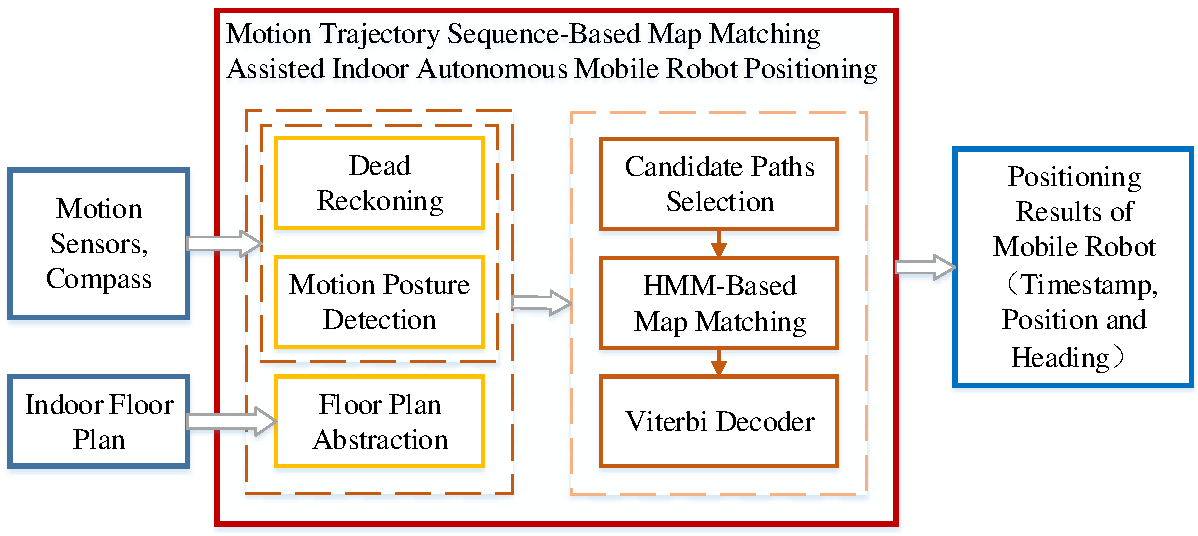
\includegraphics[width=4.8in]{RobotMatch-Architecture}
	\caption{System architecture of mobile robot positioning method.}
	\label{fig-architect}
\end{figure}

The overall architecture of mobile robot localization method presented in this paper is shown in Figure \ref{fig-architect}. The sensor data and the indoor map are used as the input of the positioning method, in which the sensor data is collected by the inertial sensors and magnetometers mounted on the mobile robot, and the indoor map is obtained by manually input or the indoor electronic map construction algorithm such as SLAM technology. The map Abstract module abstracts the indoor plane electronic map into the directed graph, the position estimation module and the motion attitude recognition module use the sensor data to give the relative position and position related action of the mobile robot respectively. The goal of map matching module is to match the motion trajectory of the mobile robot with the sequence of nodes in the directed graph, and then estimate the real time position of the mobile robot. First, the path is selected according to the direction angle estimation and the connection of the indoor path. Secondly, according to the latest alternative path and phase. The position change updates the related parameters in the hidden Markov model, and finally estimates the possibility of all the alternative paths through the online Viterbi decoder. When the matching algorithm is in the convergence stage, the most possible alternative path is the optimal estimation. The final output of the localization method proposed in this paper is the real-time location and heading of mobile robots.

\subsection{Indoor Floor Plan Abstraction}

The posture-relative positions divide the indoor path into path segments. With the path segment as a node, the action type that moves from one path segment to another path segment is a directed edge. Then the interior floor plan can be abstracted as a directed graph. Figure \ref{fig-abstract} shows an example of an interior plan and its corresponding directed graph. In this paper, a node is represented by a seven-tuple $(id,{x_1},{y_1},{x_2},{y_2},{\varphi _1},{\varphi _2})$, where ${x_i},{y_i},i = 1,2$ represent the horizontal and vertical coordinates of the two endpoints of the path segment represent the heading angle when the mobile robot moves on the path segment and reaches the corresponding endpoint. A tuple represents a directed edge between nodes, which represents the identity of the starting node, represents the identity of the terminated node,,, and represents the path from the path fragment represented by the starting node to the termination node, respectively. The horizontal, vertical coordinates, and attitude types of the relevant positions of the motion pose to which the path segment passes.

\begin{figure}[!htbp]
	\centering
	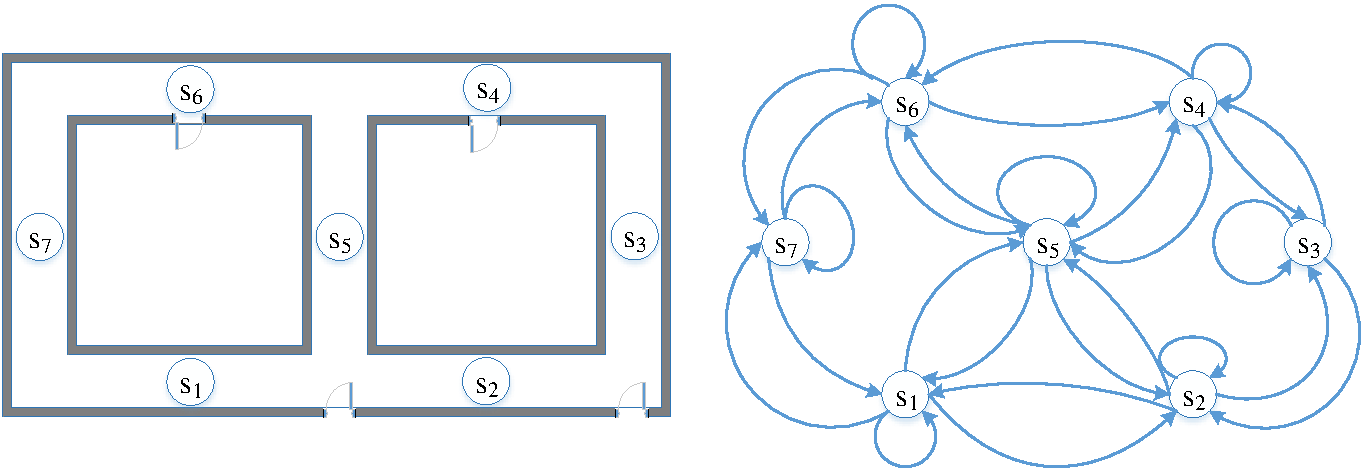
\includegraphics[width=4.576in]{RobotMatch-MapAbstract}
	\caption{Indoor floor plan abstraction example.}
	\label{fig-abstract}
\end{figure}

\subsection{Motion Posture Detection}

This section presents a decision tree model for the motion gesture recognition of indoor autonomous mobile robots. This paper focuses on the positioning of mobile robots in indoor plane maps. Therefore, this decision tree model considers only the relevant gesture recognition of the movement of a mobile robot on a plane. Including static, straight, left/right turns and U-turns.
The horizontal movement attitude of the indoor autonomous mobile robot is distinguished by different modes of the horizontal component of the accelerometer and the vertical component of the gyroscope built into the mobile robot, wherein the horizontal component of the accelerometer is the $X$-axis and Y in the local coordinate system of the robot. - The synthesis of the axis, and the vertical component of the gyroscope is the data of the Z-axis in the robot's local coordinate system, and the attitude of the mobile robot is determined by extracting the vertical component of the accelerometer. The method can be easily extended to three-dimensional indoor positioning scenes.

\begin{figure}[!htbp]
	\centering
	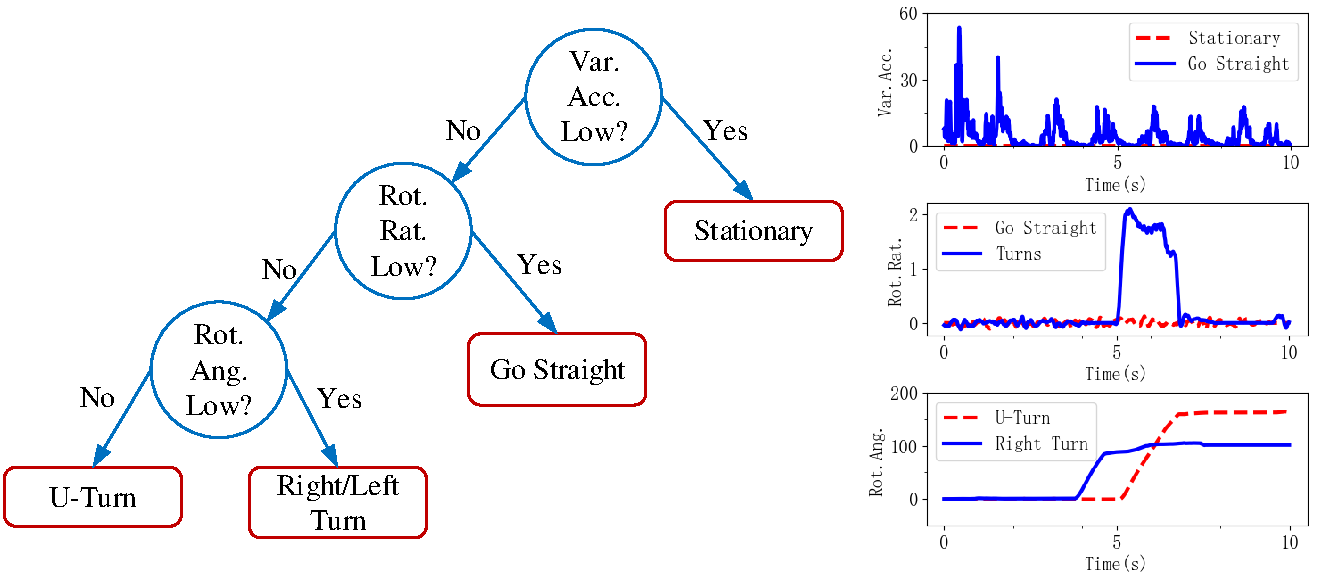
\includegraphics[width=4.95in]{RobotMatch-ActivityDecision}
	\caption{Decision tree for motion posture detection.}
	\label{fig-posture}
\end{figure}


Figure \ref{fig-posture} shows a decision tree for the motion gesture recognition of an indoor autonomous mobile robot. The decision tree uses the built-in acceleration of the mobile robot and the signal characteristics of the gyroscope data to identify different motion gestures of the mobile robot. Considering that the linear velocity of the mobile robot is obtained from the integral of the acceleration level component in time, the instantaneous velocity has an accumulated error at a certain moment. Therefore, the uppermost layer of the decision tree uses the variance of the acceleration level component to judge the mobile robot's Motion or motion, not instantaneous speed; the second level of the decision tree uses the magnitude of the rotational angular velocity measured on the Z-axis of the gyroscope to determine the straight line or turn of the mobile robot; finally, the third level of the decision tree passes through the turn process. The angle of rotation is integrated over time to obtain the rotation angle, and the rotation angle is used to distinguish whether the mobile robot is turning left/right or turning.

\begin{table}
	\label{table_conf}
	\caption{Confusion Matrix of Motion Posture Detection}
	\begin{center}
		\begin{tabular}{| c || c | c | c | c |}
			\hline
			\bfseries Motion Posture & \bfseries Left Turn & \bfseries Right Turn & \bfseries U-turn & \bfseries Go Straight\\
			\hline\hline
			\bfseries Left Turn & 58 & 0 & 2 & 0 \\
			\hline
			\bfseries Right Turn & 0 & 58 & 1 & 1 \\
			\hline
			\bfseries U-turn & 0 & 0 & 60 & 0 \\
			\hline
			\bfseries Go Straight & 0 & 0 & 0 & 60 \\
			\hline
		\end{tabular}
	\end{center}
\end{table}

In the real experimental environment, the four-wheeled differential-driving robot described in the previous paragraph was used to perform left-turning, right-turning, left-right turning, and straight-motion testing of different movement postures. Each sample was sampled for 3 seconds and each movement gesture The effective number of samples is 60. The classification results obtained by the above decision tree model are shown in Table $1$.

\section{HMM based Map Matching Algorithm}

Based on the motion posture detection based on inertial sensor data, the motion trajectory of the mobile robot can be divided into trajectory segments by left and right turn and U-turn, and these trajectory segments form a trajectory sequence in the time dimension. This section gives a detailed description of Hidden Markov Models for trajectory sequence matching to indoor abstract maps.

\subsection{Hidden Markov Model}

A Hidden Markov Model is a time-series probability model that describes the state of a process using discrete random variables. A basic HMM can be represented as $\lambda  = (S,V,A,B,\pi)$, where:

1) $S = \left\{ {{s_1},{s_2},{s_3}, \ldots ,{s_N}} \right\}$ is the set of possible states and $N = \left| S \right|$. In our case, each state represents an indoor road segment, that is, a node of the directed graph. Therefore, a state $s$ is represented by the ordered tuple in the form of ($id,x_{1},y_{1},{\varphi}_{1},x_{2},y_{2},{\varphi}_{2}$), where $id$ is the identification of road segment, $x_{1}$, $y_{1}$, ${\varphi}_{1}$, $x_{2}$, $y_{2}$ and ${\varphi}_{2}$ are different attributes of node of the directed graph, respectively. It should be noted that if the mobile robot can reach another path segment by going straight from one path segment, these two path segments can be merged into a new path segment, ie a new hidden state, as shown in Fig. 3. The path segments $s_4$, $s_6$ can be combined into new path segments.

2) $V = \left\{ {{v_1},{v_2},{v_3}, \ldots ,{v_M}} \right\}$ is the set of observations from the model and $M = \left| V \right|$. In our case, an observable state represents the relative movement distance and heading measured by an inertial sensor mounted on a mobile robot and expressed in terms of $(dist,\varphi)$.

3) $A = \left\{ {{a_{ij}}} \right\}$ is the state transition probability distribution, where \\ ${a_{ij}} = p\left\{ {{q_{t + 1}} = {s_j}|{q_t} = {s_i}} \right\}, i, j \le N$, where ${q_t}$ denotes the state at time $t$. In other words, $a_{ij}$ indicates the possibility of moving from one road segment to adjacent road segments.

4) $B = \left\{ {{b_i}(k)} \right\}$ is the observation probability distribution in state $i$, where ${b_i}(k) = p\{ {z_t} = {v_k}|{q_t} = {s_i}\},1 \le i \le N,1 \le k \le M$ and $z_t$, $q_t$ are the observation and state at time $t$, respectively. In other words, ${b_i}(k)$ indicates the possibility of a certain distance and direction measured by the inertial sensor after the mobile robot has passed a road segment.

5) $\pi  = \left\{ {{\pi _i}} \right\}$ is the initial state distribution, where ${\pi _i} = p\left\{ {{q_1} = {S_i}} \right\},1 \le i \le N$.

\subsection{Transition Probability Distribution (A)}

The transition probability distribution refers to the possibility of moving from a hidden state to the next hidden state. In this paper, the possibility of moving from one path segment to the adjacent path segment is indicated. The adjacent path segments are divided by posture-related positions. Each posture-related position has a corresponding motion posture. The higher the matching degree of the mobile robot's motion posture and position-related posture, the mobile robot passes through a path segment. The higher the probability that the gesture-related position moves to another path segment, and vice versa. Therefore, we use the degree of match between the motion pose and position-related poses of the mobile robot to represent the transition probabilities between adjacent path segments. Let the edge of the directed graph corresponding to the route segment move to the path segment be defined by section 2.3. The position-related pose corresponding to the edge is the motion pose of the mobile robot that has been identified at the given time t. The probability is shown in Equation 3, where it can be obtained from the motion pose confusion matrix in Section 2.4.
\begin{equation}
	p({s_{j,t}}|{s_{i,t - 1}}) = p({s_j}|{s_i},Ro{b_{MA}}(t)) = p(Ro{b_{MA}}(t)|{e^{ij}}.MA)
\end{equation}

\subsection{Observation Probability Distribution (B)}

In this paper, an observable state consists of the relative displacement of the mobile robot and the heading angle, and the two are independent of each other. Therefore, the observable probability distribution can be defined as:

\begin{equation}
	P({v_{k,t}}|{s_{j,t}}) = P(\varphi (t)|{s_{j,t}}) \cdot P(dist(t)|{s_{j,t}})
\end{equation}

where, $P(\varphi (t)|{s_{j,t}})$ represents the observable probability of the mobile robot's heading at time t, the condition of an implicit state, and $P(dist(t)|{s_{j,t}})$ denotes the observable probability determined by the relative displacement of the mobile robot.

The higher the degree of match between the heading of the mobile robot and the path segment, the greater the possibility that the mobile robot is located in the path segment. In the indoor environment, the error of the heading angle of the mobile robot not only comes from the accumulated error in the dead reckoning process, but also comes from the interference of various metal materials in the room with the magnetometer. In general, the error of the heading angle is relatively large. It is difficult to accurately model this error. Therefore, in this paper, Equation 5 is used to model the heading information in the observable state.

\begin{equation}
\begin{array}{l}
P(\varphi (t)|{s_{j,t}})\\
= P\{ \varphi (t)|{s_j}.{\varphi _i},i = 1,2\}  = \left\{ {\begin{array}{*{20}{l}}
	{1,if|\varphi (t) - {s_j}.{\varphi _i}| < {H_{TH}},i = 1,2}\\
	{0,others}
	\end{array}} \right.
\end{array}
\end{equation}

where, $H_{TH}$ is a constant threshold used to determine whether the heading angle of the mobile robot matches the direction of the path segment. In order to avoid that the correct path segment is excluded due to the large error of the heading angle, $H_{TH}$ is set to $59$ in this paper.

The relative displacement error of the mobile robot mainly comes from the accumulative error caused by the acceleration error in the dead reckoning process. Here we assume that the relative displacement of the mobile robot obeys the Gaussian distribution. On the one hand, intuitively speaking, the closer the relative displacement of the mobile robot is to the length of the path segment, the more likely the mobile robot is located in the path segment; on the other hand, the length of the path segment is much larger than the relative displacement of the mobile robot. All path fragments should have similar possibilities. Combining the above two conditions, this paper uses Equation 6 to model the relative displacement information in the observable state.

\begin{equation}
\begin{array}{l}
P(dist(t)|{s_{j,t}})\\
= P\{ dist(t)|{s_j}.dist\}  = \left\{ {\begin{array}{*{20}{l}}
	{\frac{1}{{\sqrt {2\pi } {\sigma _d}}}{e^{ - 4.5}},dist(t) + 3{\sigma _d} \le {s_j}.dist}\\
	{\frac{1}{{\sqrt {2\pi } {\sigma _d}}}{e^{ - \frac{{{{(dist(t) - {s_j}.dist)}^2}}}{{2{\sigma _d}^2}}}},others}
	\end{array}} \right.
\end{array}
\end{equation}

Where ${s_j}.dist$ is the length of the path segment, which can be derived from the two endpoints of the path segment, which is the standard deviation of the relative movement distance of the mobile robot at time t. In order to estimate the value, this paper first tests the change of the accelerometer's value when the mobile robot is at rest, and estimates the standard deviation of the acceleration based on the absolute median error (MAD) of the test data. The principle of the dead reckoning described in Section 2.1 is used. It can be inferred that there is a secondary relationship with [18].

\begin{equation}
	{\sigma _a} = 1.4826 \times median(\left| {\Delta a} \right|)
\end{equation}

\subsection{Initial State Distribution}

If the starting point of the mobile robot is known, then the path segment where the starting point is located is the initial state, and the probability is set to 1; if the starting point of the moving robot is unknown, all can be selected by formula 5 based on the initial heading information of the moving robot. For possible alternative path segments, the initial probability distribution is a uniform distribution over the candidate path segments. Correspondingly, the starting point of the mobile robot is assumed to be the average of the starting points of all candidate path segments. In this paper, the initial heading angle of a mobile robot can be obtained from a digital compass or set manually.

\subsection{Optimal Motion Trajectory Estimation}

Based on the above-defined Hidden Markov Model, this paper uses Viterbi algorithm to determine the optimal estimation of the moving trajectory of a mobile robot. For a given observable state sequence $({z_1},{z_2},...,{z_k})$, the goal of the Viterbi algorithm is to find the most hidden State sequence $({q_1},{q_2},...,{q_k})$. Fig. \ref{fig-viterbi} briefly illustrates the decoding process of the Viterbi algorithm.

\begin{figure}[!htbp]
	\centering
	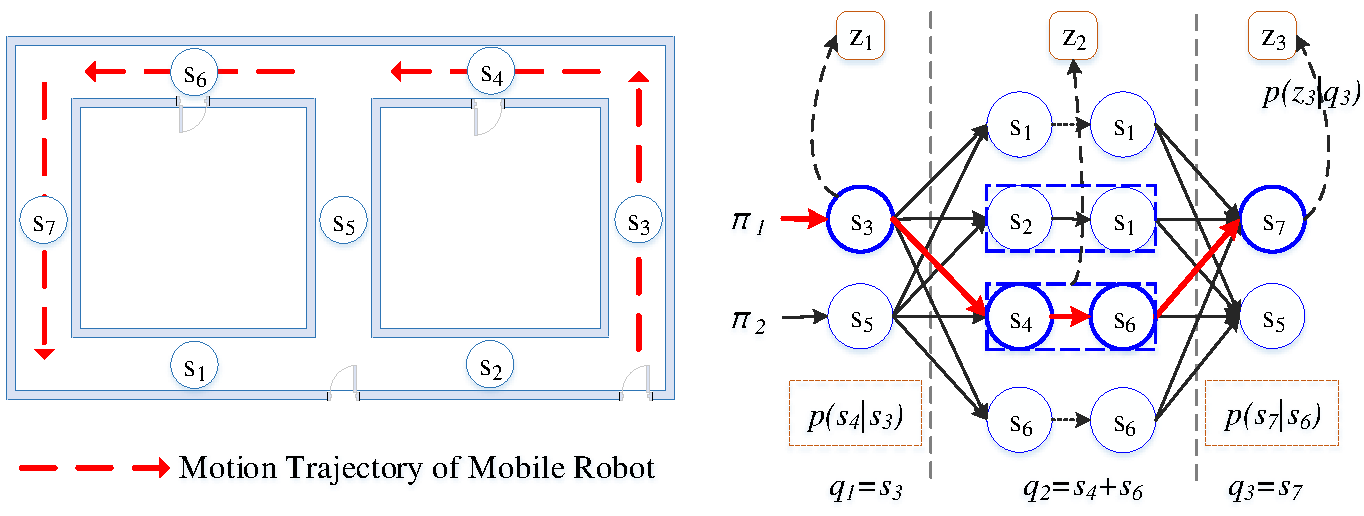
\includegraphics[width=4.976in]{RobotMatch-ViterbiDecoding}
	\caption{Illustration of the proposed HMM model Viterbi decoding.}
	\label{fig-viterbi}
\end{figure}

The Viterbi decoder is implemented by the dynamic programming method. First, a Viterbi variable is defined to represent the maximum probability that the Hidden Markov Model will reach the state along a path at time t and output:

\begin{equation}
	{\delta _t}(i) = \max P\{ {q_1},{q_2}, \cdots ,{q_t} = {s_i},{z_1},{z_2}, \cdots ,{z_t}|\lambda \}
\end{equation}

At time $t+1$, the maximum probability reaching the hidden state $s_j$ can be recursively derived from the Viterbi variable at time $t$ by the following equation. 
\begin{equation}
	{\delta _{t + 1}}(j) = [\mathop {\max }\limits_i ({\delta _t}(i) \cdot P\{ {q_{t + 1}} = {s_i}|{q_t} = {s_j}\} )] \cdot P\{ {z_{t + 1}}|{q_{t + 1}}\} ,1 \le t \le k
\end{equation}

By recording the back-pointer, at time k, the most likely hidden state sequence, that is, the optimal estimation of the moving trajectory of the mobile robot can be obtained by the path backtracking method. Algorithm $1$ summarizes the processing flow of the trajectory sequence map matching method presented in this paper.

AiFiMatch algorithm is summarized with the pseudocode in Algorithm \ref{alg_aifi}.  

\begin{algorithm}[H]
	\caption{Motion trajectory sequence-based map matching algorithm}
	\label{alg_aifi}
	\begin{algorithmic}[1]
		
		\renewcommand{\algorithmicrequire}{\textbf{Input:}}
		\renewcommand{\algorithmicensure}{\textbf{Output:}}
		\REQUIRE Sensor data up to current time t: $data_{1:t}$
		\REQUIRE Abstraction of indoor floor plan: $fp$
		\ENSURE Optimal state sequence estimation at current time $t$: $Q_t$
		\ENSURE Mobile robot's position and posture estimation at current time $t$: ${Rob}_t$
		
		\renewcommand{\algorithmicrequire}{\textbf{Define:}}
		\REQUIRE Starting time of current sub-trajectory: $st$, the initial value of $st$ is $0$
		\REQUIRE Length of current motion trajectory sequence: $k$, the initial value of $k$ is $1$
		\REQUIRE Array of Viterbi variables and backward pointers: ${Vtb}_{k}(t)$
		\REQUIRE Candidate road segment list at current time: $S(t)$
		
		
		\STATE ${{Rob}_{t}.{MA}}, at \leftarrow Posture\_Detect({data_{1:t}})$
		
		\IF{${{Rob}_{t}.{MA}}\ != \ None$}  
		
			\STATE ${st} \leftarrow {at}$  
			
			\STATE // Calculate the transition probability TR[ ][ ]
			\FOR{$s_i\ in\ S(t-1)$}
			\STATE $S^i(t) \leftarrow Candidate\_Select(fp, s_i)$
			\FOR{$s_j\ in\ S^i(t)$}
			\STATE TR[i][j] $\leftarrow p(s_j|s_i,Rob_t.MA)$
			\ENDFOR
			\STATE $S(t).extend(S_i(t))$
			\ENDFOR
			
			\STATE // Calculate the observation probability OB[ ]
			\STATE $z(t) \leftarrow Dead\_Reckoning(data_{st:t})$
			\FOR{$s_i\ in\ S(t)$}
			\STATE OB[i] $\leftarrow p(z(t)|s_i)$
			\ENDFOR
			\STATE $Vtb_{k+1}(t) \leftarrow Viterbi\_Calculate(Vtb_{k}(t-1)$, OB[ ], TR[ ][ ]$)$
			\STATE $k$+=1
		
		\ELSE // Not a position-related posture
		
			\STATE // Calculate the observation probability OB[ ]
			\STATE $z(t) \leftarrow Dead\_Reckoning(data_{st:t})$
			\STATE $S(t) \leftarrow S(t-1)$
			\FOR{$s_i\ in\ S(t)$}
			\STATE OB[i] $\leftarrow p(z(t)|s_i)$
			\ENDFOR
			
			\STATE $Vtb_{k}(t) \leftarrow Viterbi\_Calculate(Vtb_{k}(t-1)$, OB[ ]$)$
			
		\ENDIF
		
		\STATE $Q_t \leftarrow Viterbi\_Decoder(Vtb_{k}(t))$
		\STATE $Rob_t \leftarrow Update\_Estimation(data_{st:t}, Q_t)$
		
		\State return $Q_t, Rob_t$
	\end{algorithmic}
\end{algorithm}


\section{Evaluation}

We uses the wheel mobile robot introduced in Section 2 to complete the experimental analysis. The experimental environment is part of the fifth floor of the experimental building of the author. The experimental area is divided into east and west parts, and the east part is approximately 84.85 * 66.8 square meters. The west part is approximately 68.7 * 106.75 square meters, the connecting corridor length is 46.25 meters and the width is 2.4 meters. The overall layout is shown in Figure 6. In order to record the real position of the robot during the movement, this article divides the experimental area into squares of 0.8 * 0.8 square meters and marks. In the experiment process, another intelligent vehicle with camera function is used to move in parallel with the robot. Real-time recording of the location. In the experimental area, the robot moves along the two planned paths in Figure 6 and is denoted as $T_1$ and $T_2$, respectively. The length of $T_1$ is 181.9 meters, including 3 position related positions. The whole trajectory is divided into 3 trajectory-related trajectories divided into 4 trajectory sub-tracks; $T_2$ length is 180.5 meters, including 2 posture related positions, the whole trajectory is 2 The position-related poses are divided into three trajectories consisting of sub-tracks, and the robot is repeated $9$ times for each path.

\begin{figure}[!htbp]
	\centering
	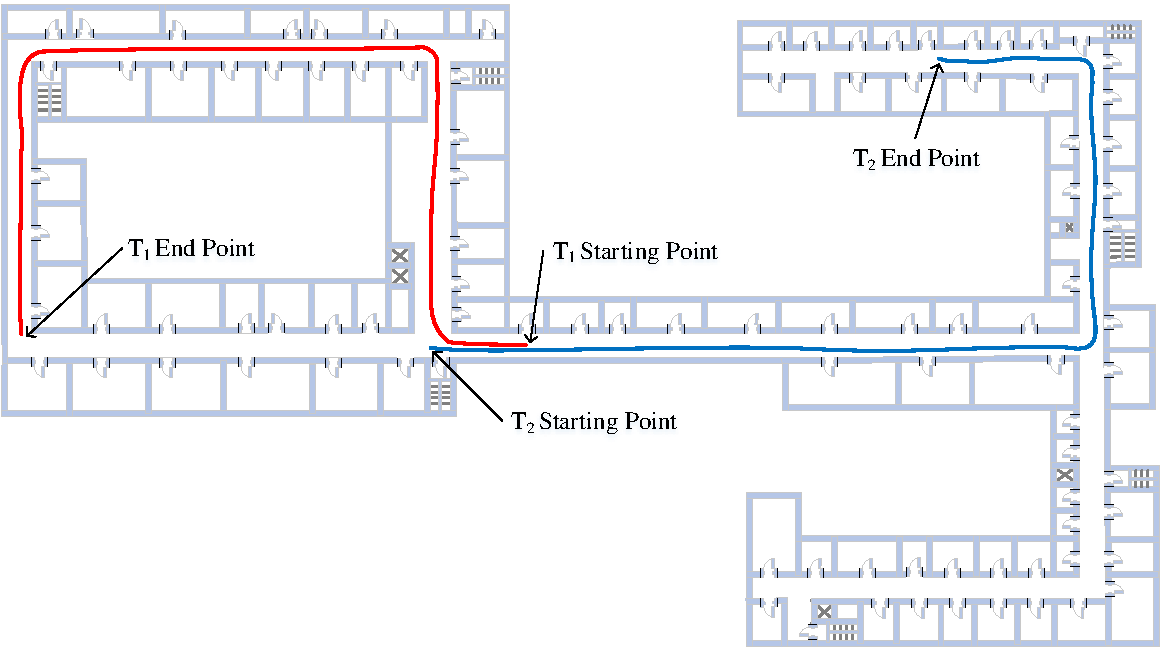
\includegraphics[width=4.976in]{RobotMatch-Environment}
	\caption{Indoor floor plan of experimental environment and mobile robot trajectories.}
	\label{fig-environment}
\end{figure}

\subsection{Influence of Heading Direction Errors}

When the starting point is unknown, the convergence performance of the algorithm is closely related to the recognition results of position-related gestures. In general, after at least two consecutive position-recognition gestures need to be correctly recognized, the map matching algorithm based on the gesture recognition is likely to converge. , And correspondingly, in the process of position-related gesture recognition (such as left and right turning) facing indoor plane maps, the error of the heading angle has a greater impact on the attitude recognition results. Therefore, this section first analyzes the heading angle error for the proposed text. The influence of the convergence performance of map matching algorithm. Here, we first define the correct rate of position-related gesture recognition by Equation 10.

\begin{equation}
	{Precison} = \frac{Number\ of\ Correctly\ Detected\ Consecutive\ Two\ Postures}{Total\ Number\ of\ Consecutive\ Two\ Postures}
\end{equation}

Assume that the distribution of the heading angle estimation error is Gaussian and the average is 0. Based on the original data of the heading angle, a Gaussian distribution-based random number is added to simulate different degrees of error. Figure 7 shows the errors at different heading angles. The variation of the correct rate of position-dependent gesture recognition under the condition of the standard deviation of the distribution. It can be seen from Fig. 7 that the accuracy of position-dependent gesture recognition is stable under certain heading angle error conditions, but when the standard deviation of the error distribution reaches a certain level (T1 is 40 degrees and T2 is 30 degrees), The correct rate dropped rapidly.

\begin{figure}[!htbp]
	\centering
	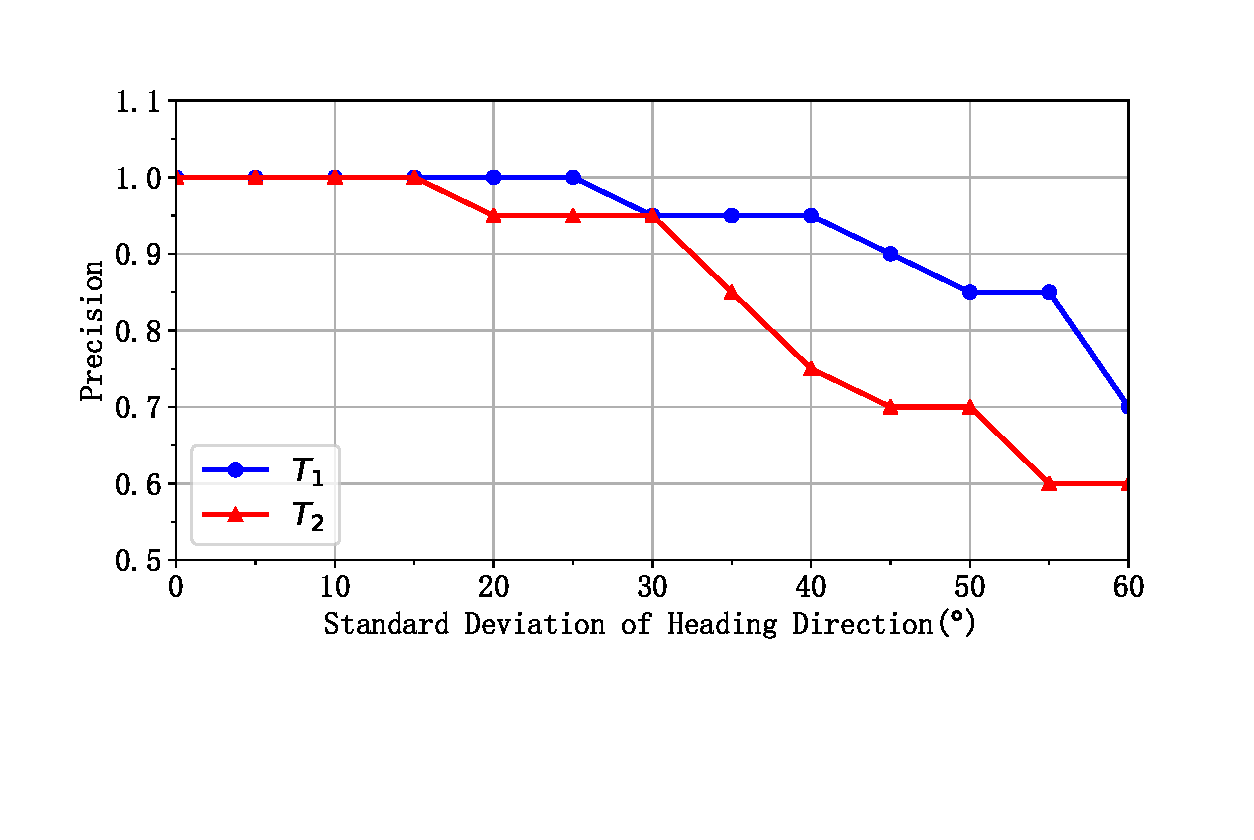
\includegraphics[width=3.976in]{RobotMatch-HeadingError}
	\caption{Heading errors on the precision of mobile robot posture detection.}
	\label{fig-headingerror}
\end{figure}

\subsection{Convergence Speed Analysis without Knowing the Starting Point}

Under the condition that the starting point is unknown, after the mobile robot moves a certain distance, the algorithm can still converge and finally estimate the real-time position of the mobile robot. The distance before the convergence of the algorithm shows the convergence performance of the algorithm. In order to evaluate the convergence performance of the proposed map matching algorithm, we compare the proposed map matching algorithm with the semimatch algorithm proposed in [18]. The semMatch algorithm has certain similarities with the algorithm presented in this paper. The hidden Markov model is also used to implement map matching operations. However, the details of the model are slightly different.

\begin{figure}[!htbp]
	\centering
	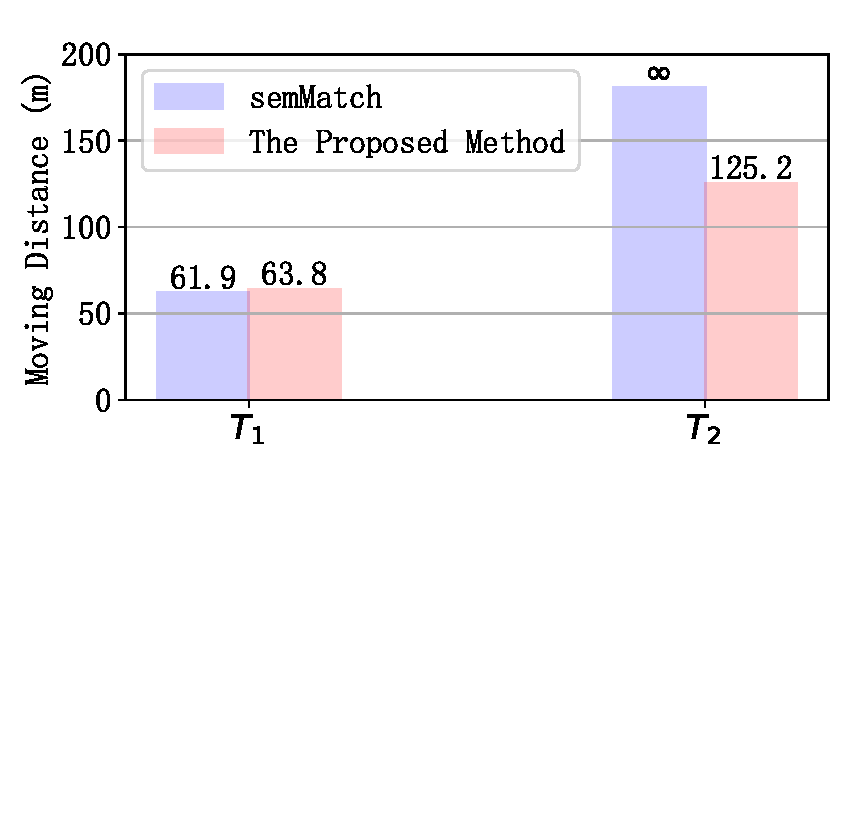
\includegraphics[width=3.276in]{RobotMatch-Convergence}
	\caption{Distance traveled before convergence for each trajectory.}
	\label{fig-convergence}
\end{figure}

Using the same decision tree model to identify the pose types in the trajectory of a moving robot, Figure 8 shows the convergence of the two algorithms. On the one hand, for the T1 path, both algorithms reach the convergence state after passing through two pose-related positions. However, the algorithm proposed in this paper needs to observe the subsequent path segment after identifying the corresponding pose type, so the convergence performance is improved. Slightly worse, when it reaches the convergence state, the mobile robot moves 1.9 meters more. On the other hand, for the T2 path, the algorithm proposed in this paper reaches the convergence state shortly after the recognition of the first position-related pose, and the corresponding seamatch algorithm does not converge due to the symmetry of the interior structure. The infinity is denoted by the infinity large size ∞. The main reason is the difference in the model definition of the two map matching algorithms. The implicit state of the map matching algorithm proposed in this paper is the straight line segment in the indoor road network. In the T2 path, the mobile robot Firstly, a path segment with a long enough length is combined with the subsequent recognition of the first position-related pose to achieve the convergence of the algorithm.


\subsection{Online Positioning Performance with Knowing the Starting Point}

Under the condition that the starting point is known, the localization algorithm proposed in this paper does not need to pass the motion trajectory matching stage to converge. After convergence, the algorithm can track the moving trajectory of the mobile robot in real time. We use the Euler distance between the real physical position of the autonomous mobile robot and the position estimate given by the algorithm to analyze the real-time positioning performance. Figure 9 shows the positioning of autonomous mobile robots with increasing distances on both T1 and T2 paths. Error variation.

\begin{figure}[!htbp]
	\centering
	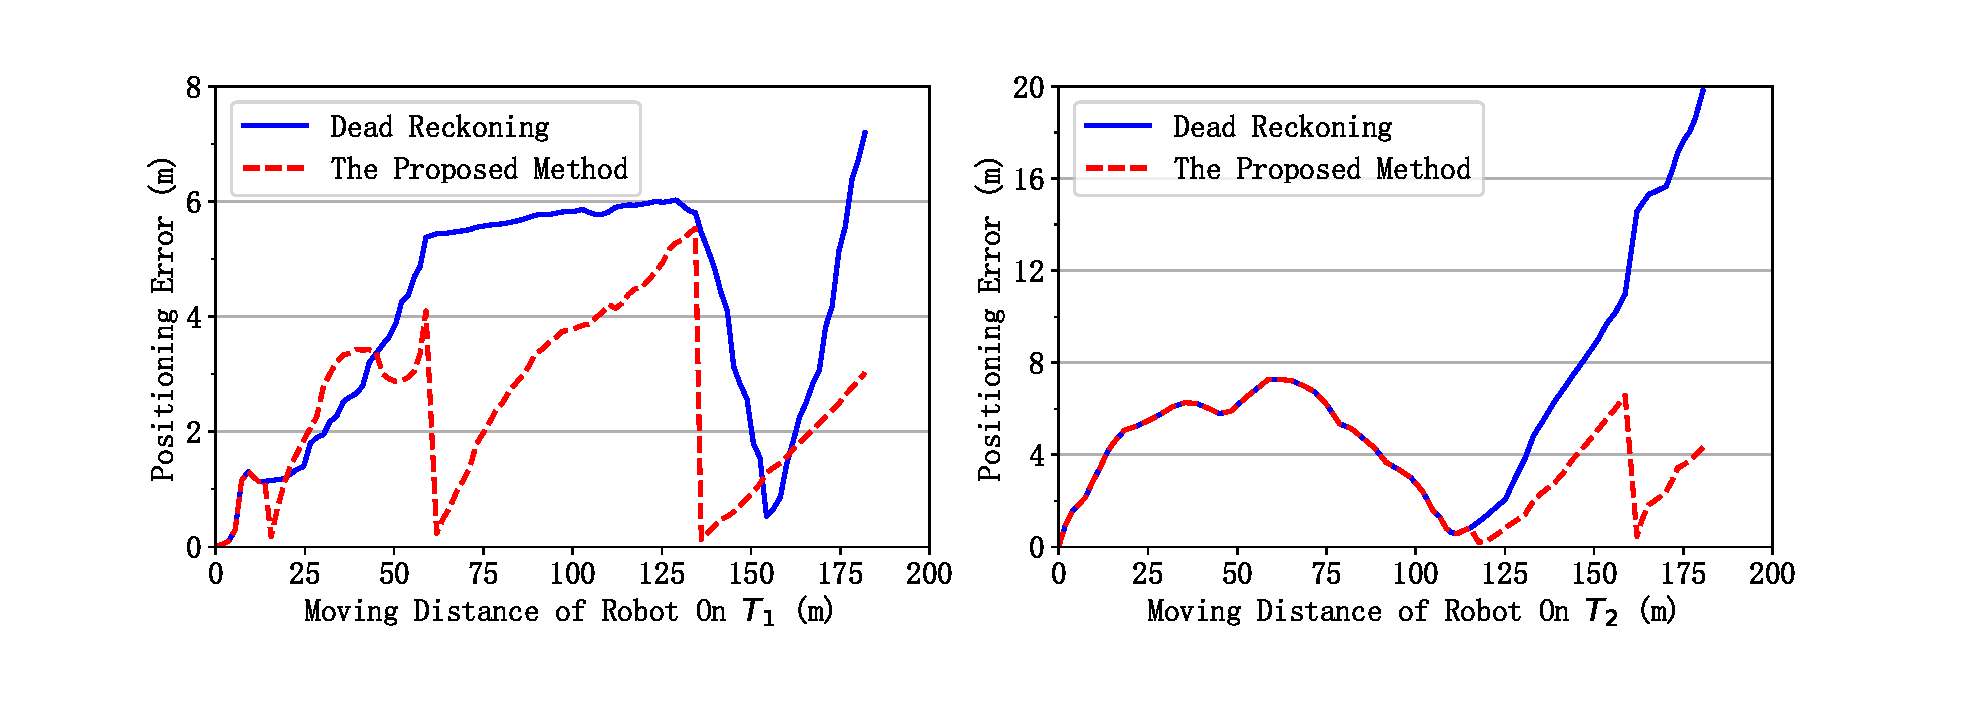
\includegraphics[width=5.076in]{RobotMatch-OnlineError}
	\caption{Online positioning errors for each trajectory.}
	\label{fig-online}
\end{figure}

When the motion trajectory does not include posture related position, the map matching assisted positioning technology proposed in this paper is equivalent to the traditional dead reckoning technology, but after identifying the relevant position of the pose, the coordinates of the known pose related position can be used to move the coordinates. The real-time position of the robot is corrected. The real-time positioning results of the mobile robot on the two paths T1 and T2 shown in Fig. 9 are verified by the positioning results on both paths. For the T1 path, the average positioning error is 4.0. The meter falls to 2.49 meters, while for the T2 path, the average positioning error decreases from 6.58 meters to 3.39 meters. From the above trend, it can be deduced that in the actual environment, the greater the density of posture-related locations, the more obvious the improvement of the traditional dead reckoning technology is.


\subsection{Influence of Acceleration Errors}

From the principle of dead reckoning technology described in section 2.1 of this paper, we know that the acceleration error has a quadratic relationship with the error of the moving distance of the mobile robot. Therefore, the acceleration error is one of the main sources of accumulated error in dead reckoning technology. This section simulates different acceleration error scenarios by adding Gaussian random generation numbers of different standard deviations to the original acceleration data, and then analyzes the influence of the acceleration error on the positioning algorithm proposed in this paper.

\begin{figure}[!htbp]
	\centering
	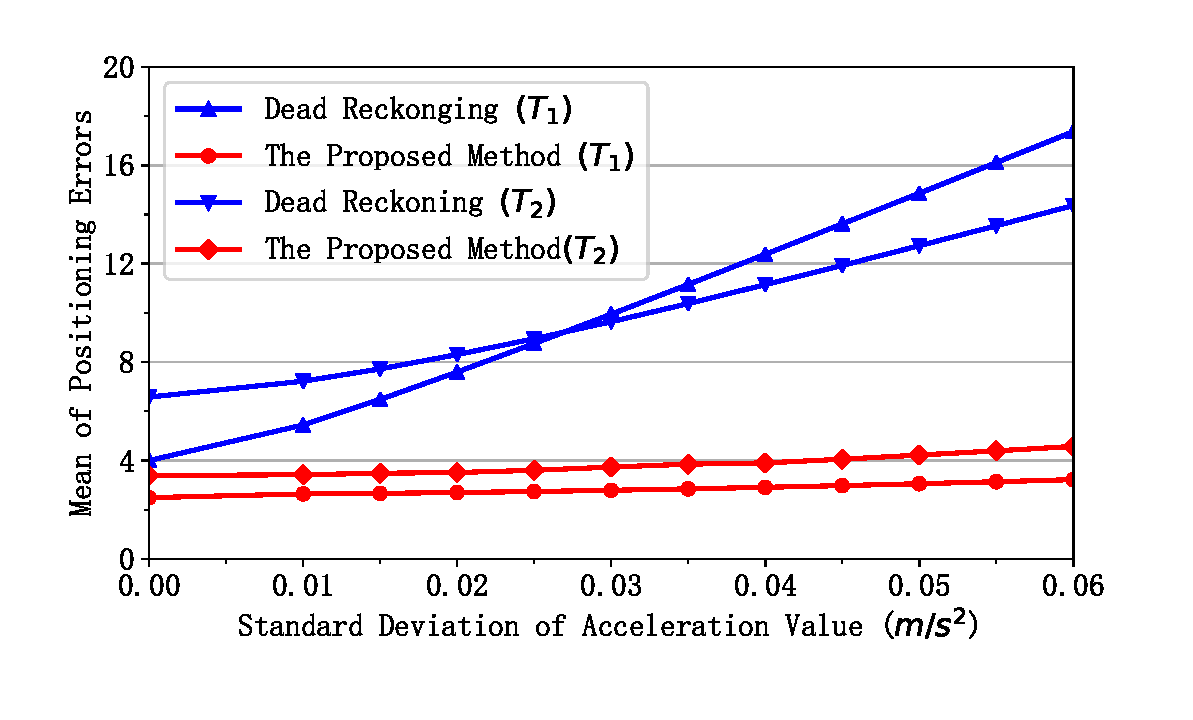
\includegraphics[width=3.676in]{RobotMatch-AcceError}
	\caption{Acceleration value errors on the mean of positioning errors for each trajectory.}
	\label{fig-acce-error}
\end{figure}

Fig. \ref{fig-acce-error} shows the average positioning error of the mobile robots in the two paths T1 and T2 under different standard deviation values. It can be seen from the figure that, on the one hand, based on a slight increase in the acceleration error, the dead reckoning is based on dead reckoning. The positioning method of the technique rapidly increases the average positioning error, which means that the positioning performance of dead reckoning technology is very sensitive to the acceleration error; on the other hand, compared with the traditional dead reckoning technology, the same acceleration error changes. The positioning error of the positioning algorithm proposed in this paper changes more smoothly, which shows that the positioning algorithm has a certain degree of robustness to the acceleration error.
 

\section{Conclusion}

In order to solve the difficult problem of positioning of autonomous mobile robots in dark complex building corridors, subway tunnels, or underground mines after sudden accident such as a fire, this paper proposes an indoor autonomous mobile robot tracking and positioning algorithm based on a novel hidden Markov Model. In the structured indoor environment, this method uses the detection of position-related postures to match the motion trajectory of mobile robot to the abstraction of indoor floor plan. Compared with the traditional dead reckoning technology, the proposed algorithm can significantly reduce the influence of cumulative errors on the positioning accuracy, and is robust to the heading direction and acceleration value noises within a certain error range. This algorithm does not rely on cameras, and uses only motion sensors installed in autonomous mobile robots and known indoor floor plan to achieve fusion positioning of dead reckoning and map matching techniques, even when the starting point is unknown. This algorithm has the characteristics of simple deployment, low manufacturing cost, and easy operation.

%
% ---- Bibliography ----
%
\bibliographystyle{splncs}
%\bibliographystyle{splncs03_unsrt}
%\bibliographystyle{unsrt}
%% ------ update by springer lncs ----- %%
%\bibliographystyle{splncs04}
\bibliography{RobotMatch}

\end{document}
